\onecolumn
\subsection{Additional plots and graphs}\label{app:B}
\begin{figure*}[ht]
	\centering
	
\includegraphics[width=\textwidth]{fig/Model_Comparison_Price_MAE.png}
	\caption{Comparison of the best performing model at each horizon for the 
	delta target. Constellations of training data that
		achieved the best performance of each model differs depending on model 
		and horizon. Lower is better.}
	\label{fig:modelComparisonPrice}
\end{figure*}

\begin{figure*}[ht]
	\centering
	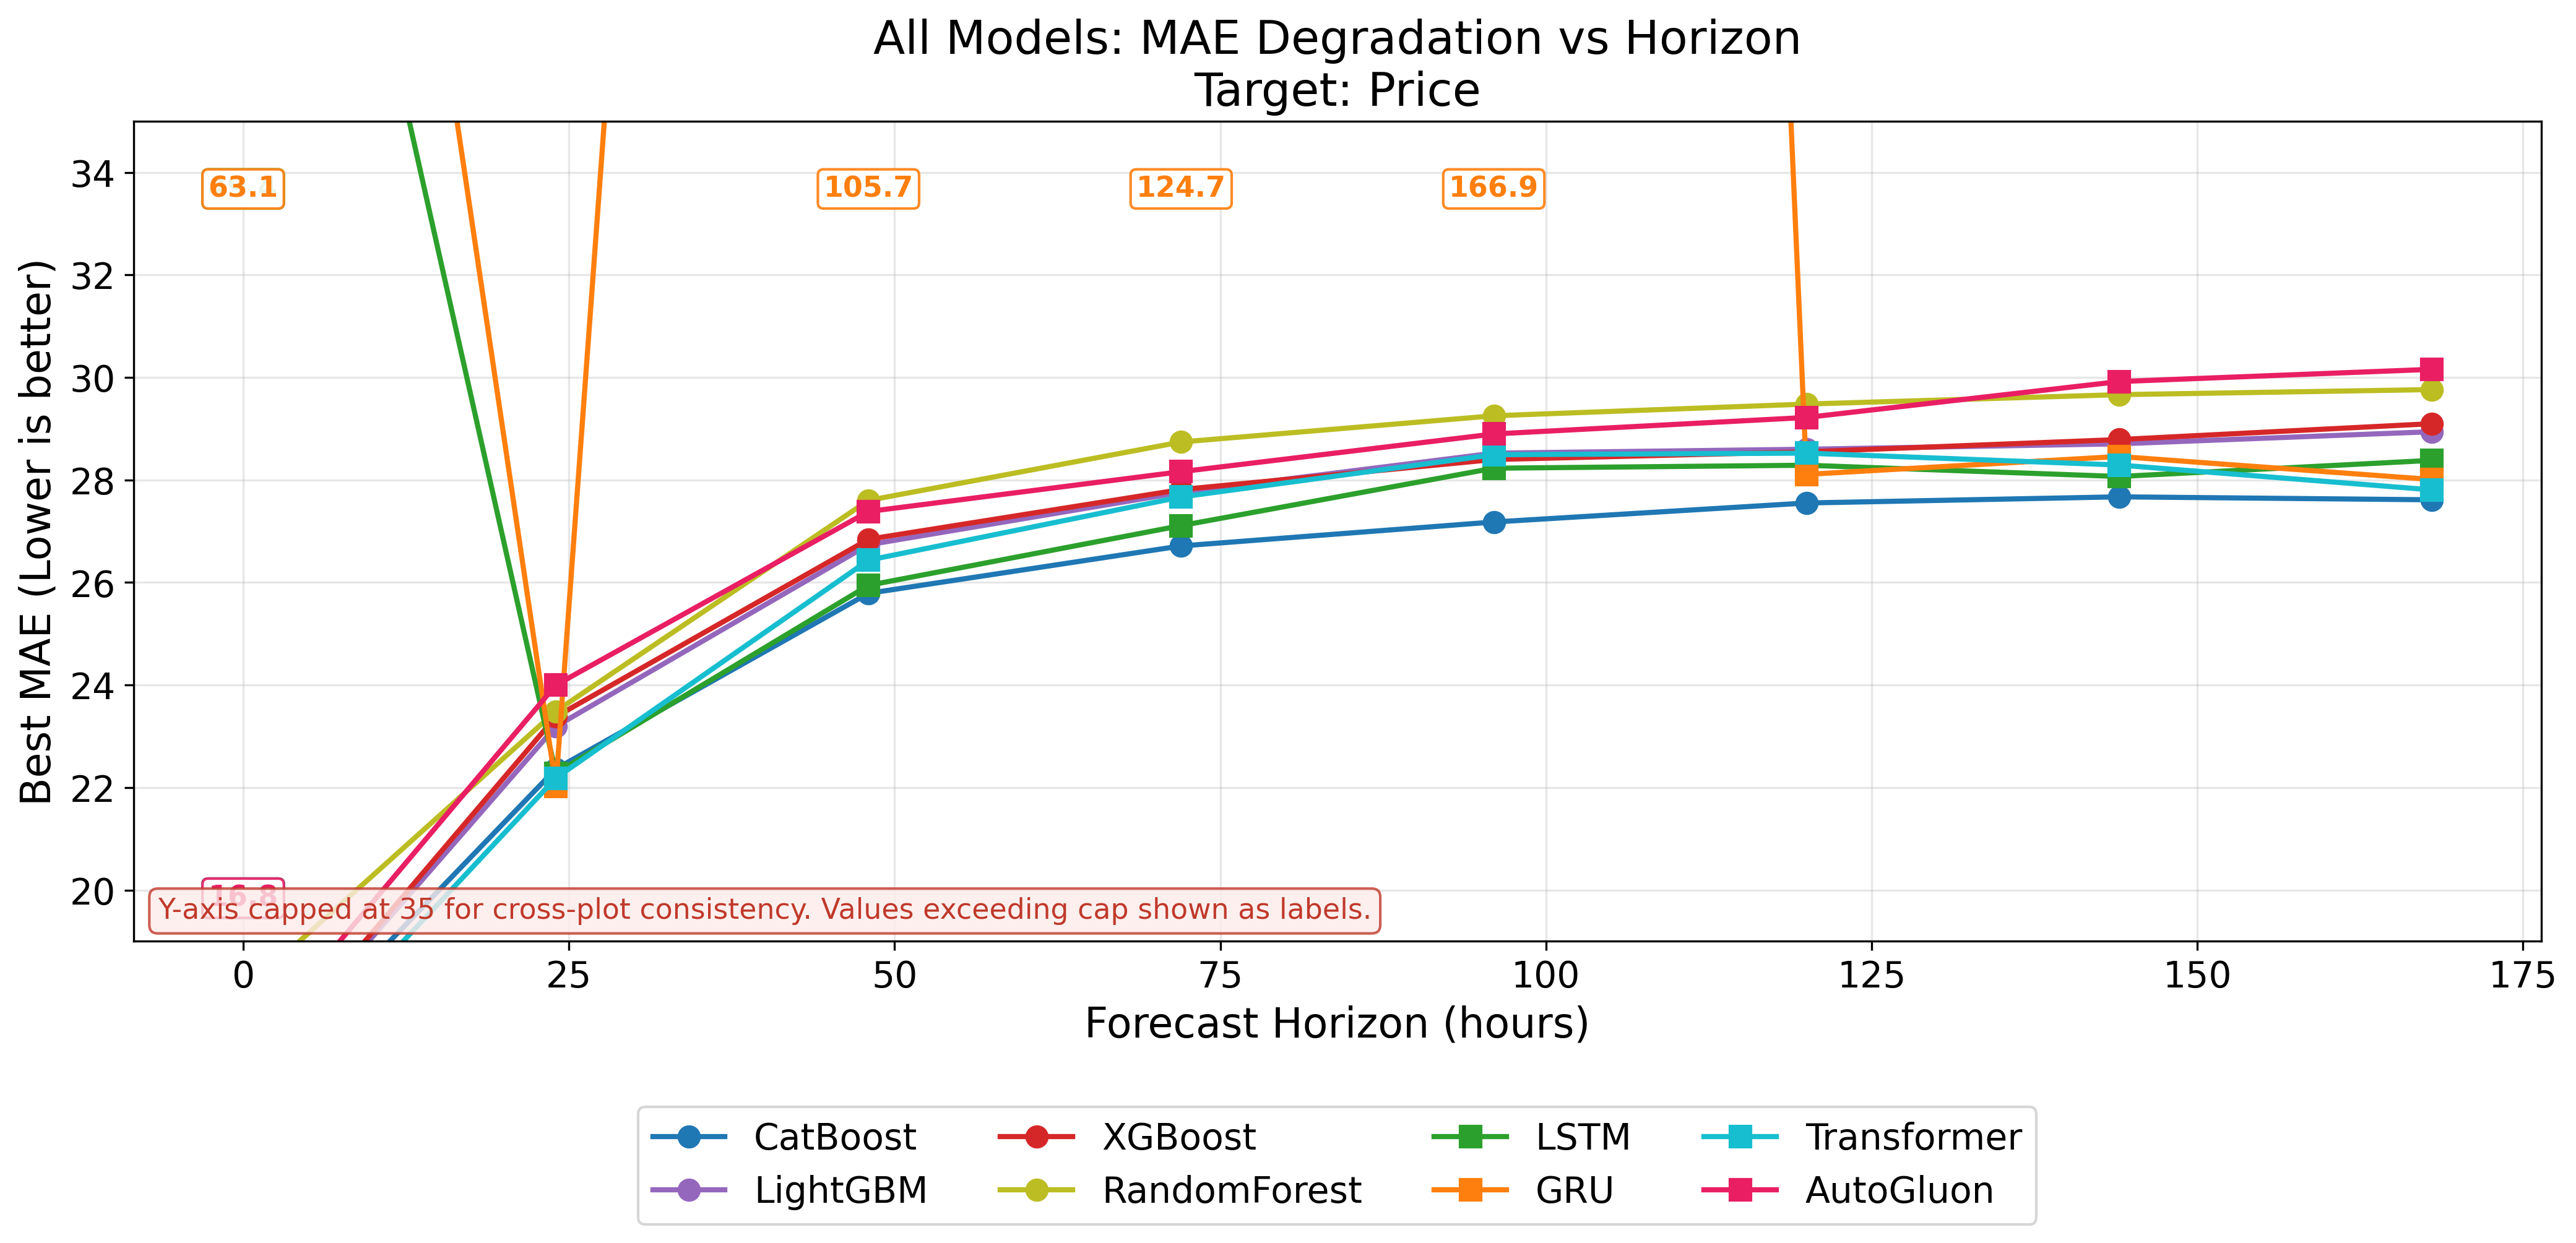
\includegraphics[width=\textwidth]{fig/Horizon_Degradation_All_Price_MAE.png}
	\caption{ Graph showing how each of the architectures degrade as the 
	forecasting horizon is expanded. Lower is better.}
	\label{fig:horizonDegredationPrice}
\end{figure*}

\begin{figure*}[ht]
	\centering
	
\includegraphics[width=\textwidth]{fig/Pruning_Gain_Delta_MAE.png}
	\caption{Visualization of pruning impact. Upwards bars indicate improvement 
	in performance after pruning.}
	\label{fig:pruningGainDelta}
\end{figure*}

\begin{figure*}[ht]
	\centering
	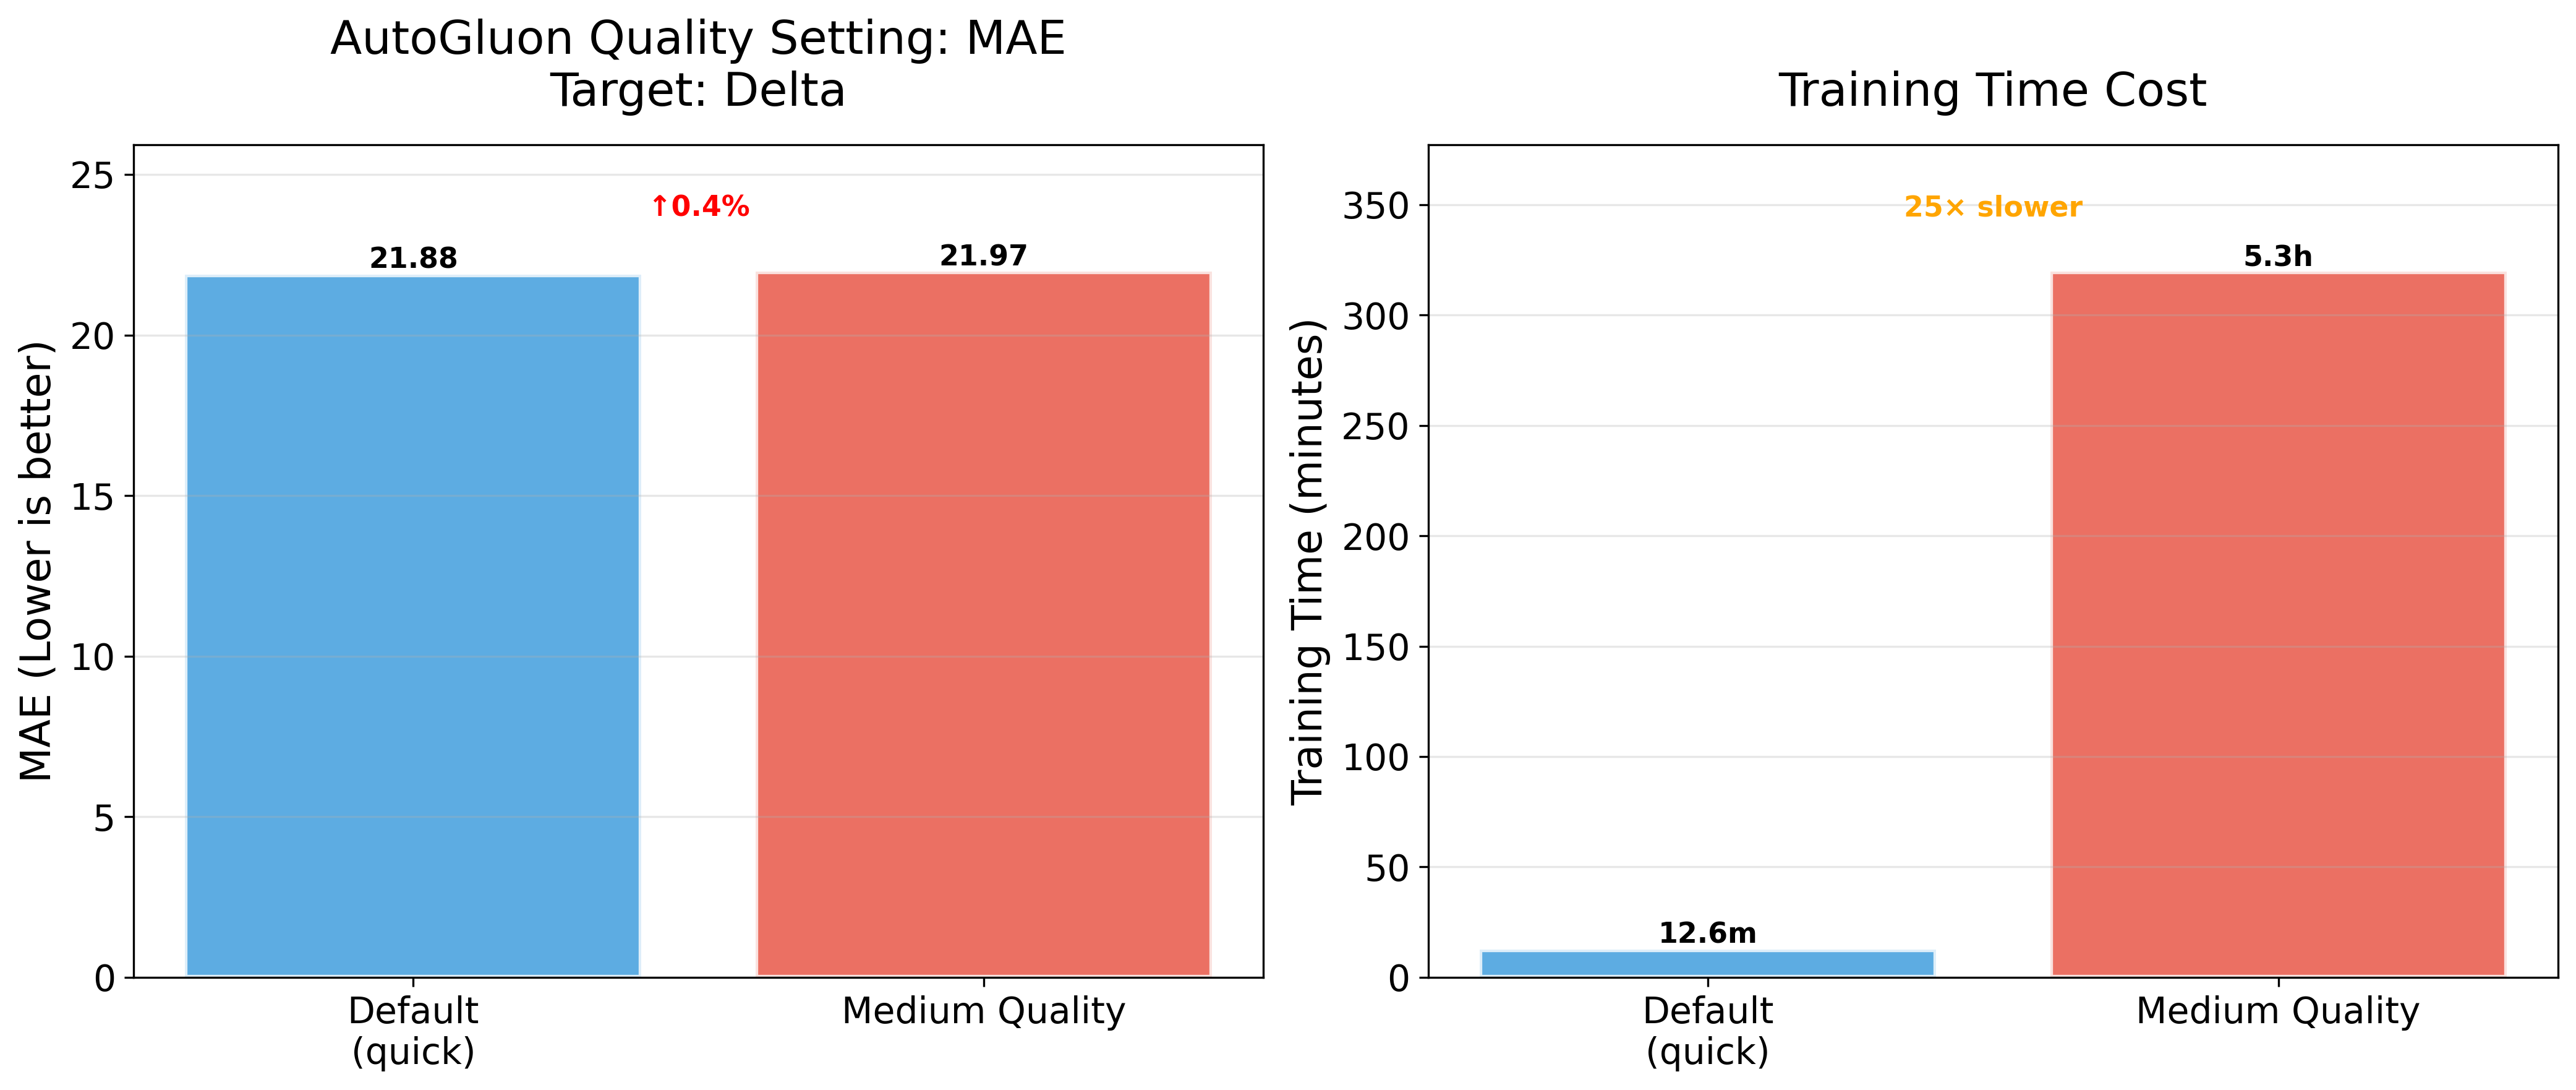
\includegraphics[width=\textwidth]{fig/AutoGluon_Quality_Tiers_Delta.png}
	\caption{ MAE and training time comparison between the fast and medium 
	AutoGluon presets. Lower is better.}
	\label{fig:autoGluonDelta}
\end{figure*}

\begin{figure*}[ht]
	\centering
	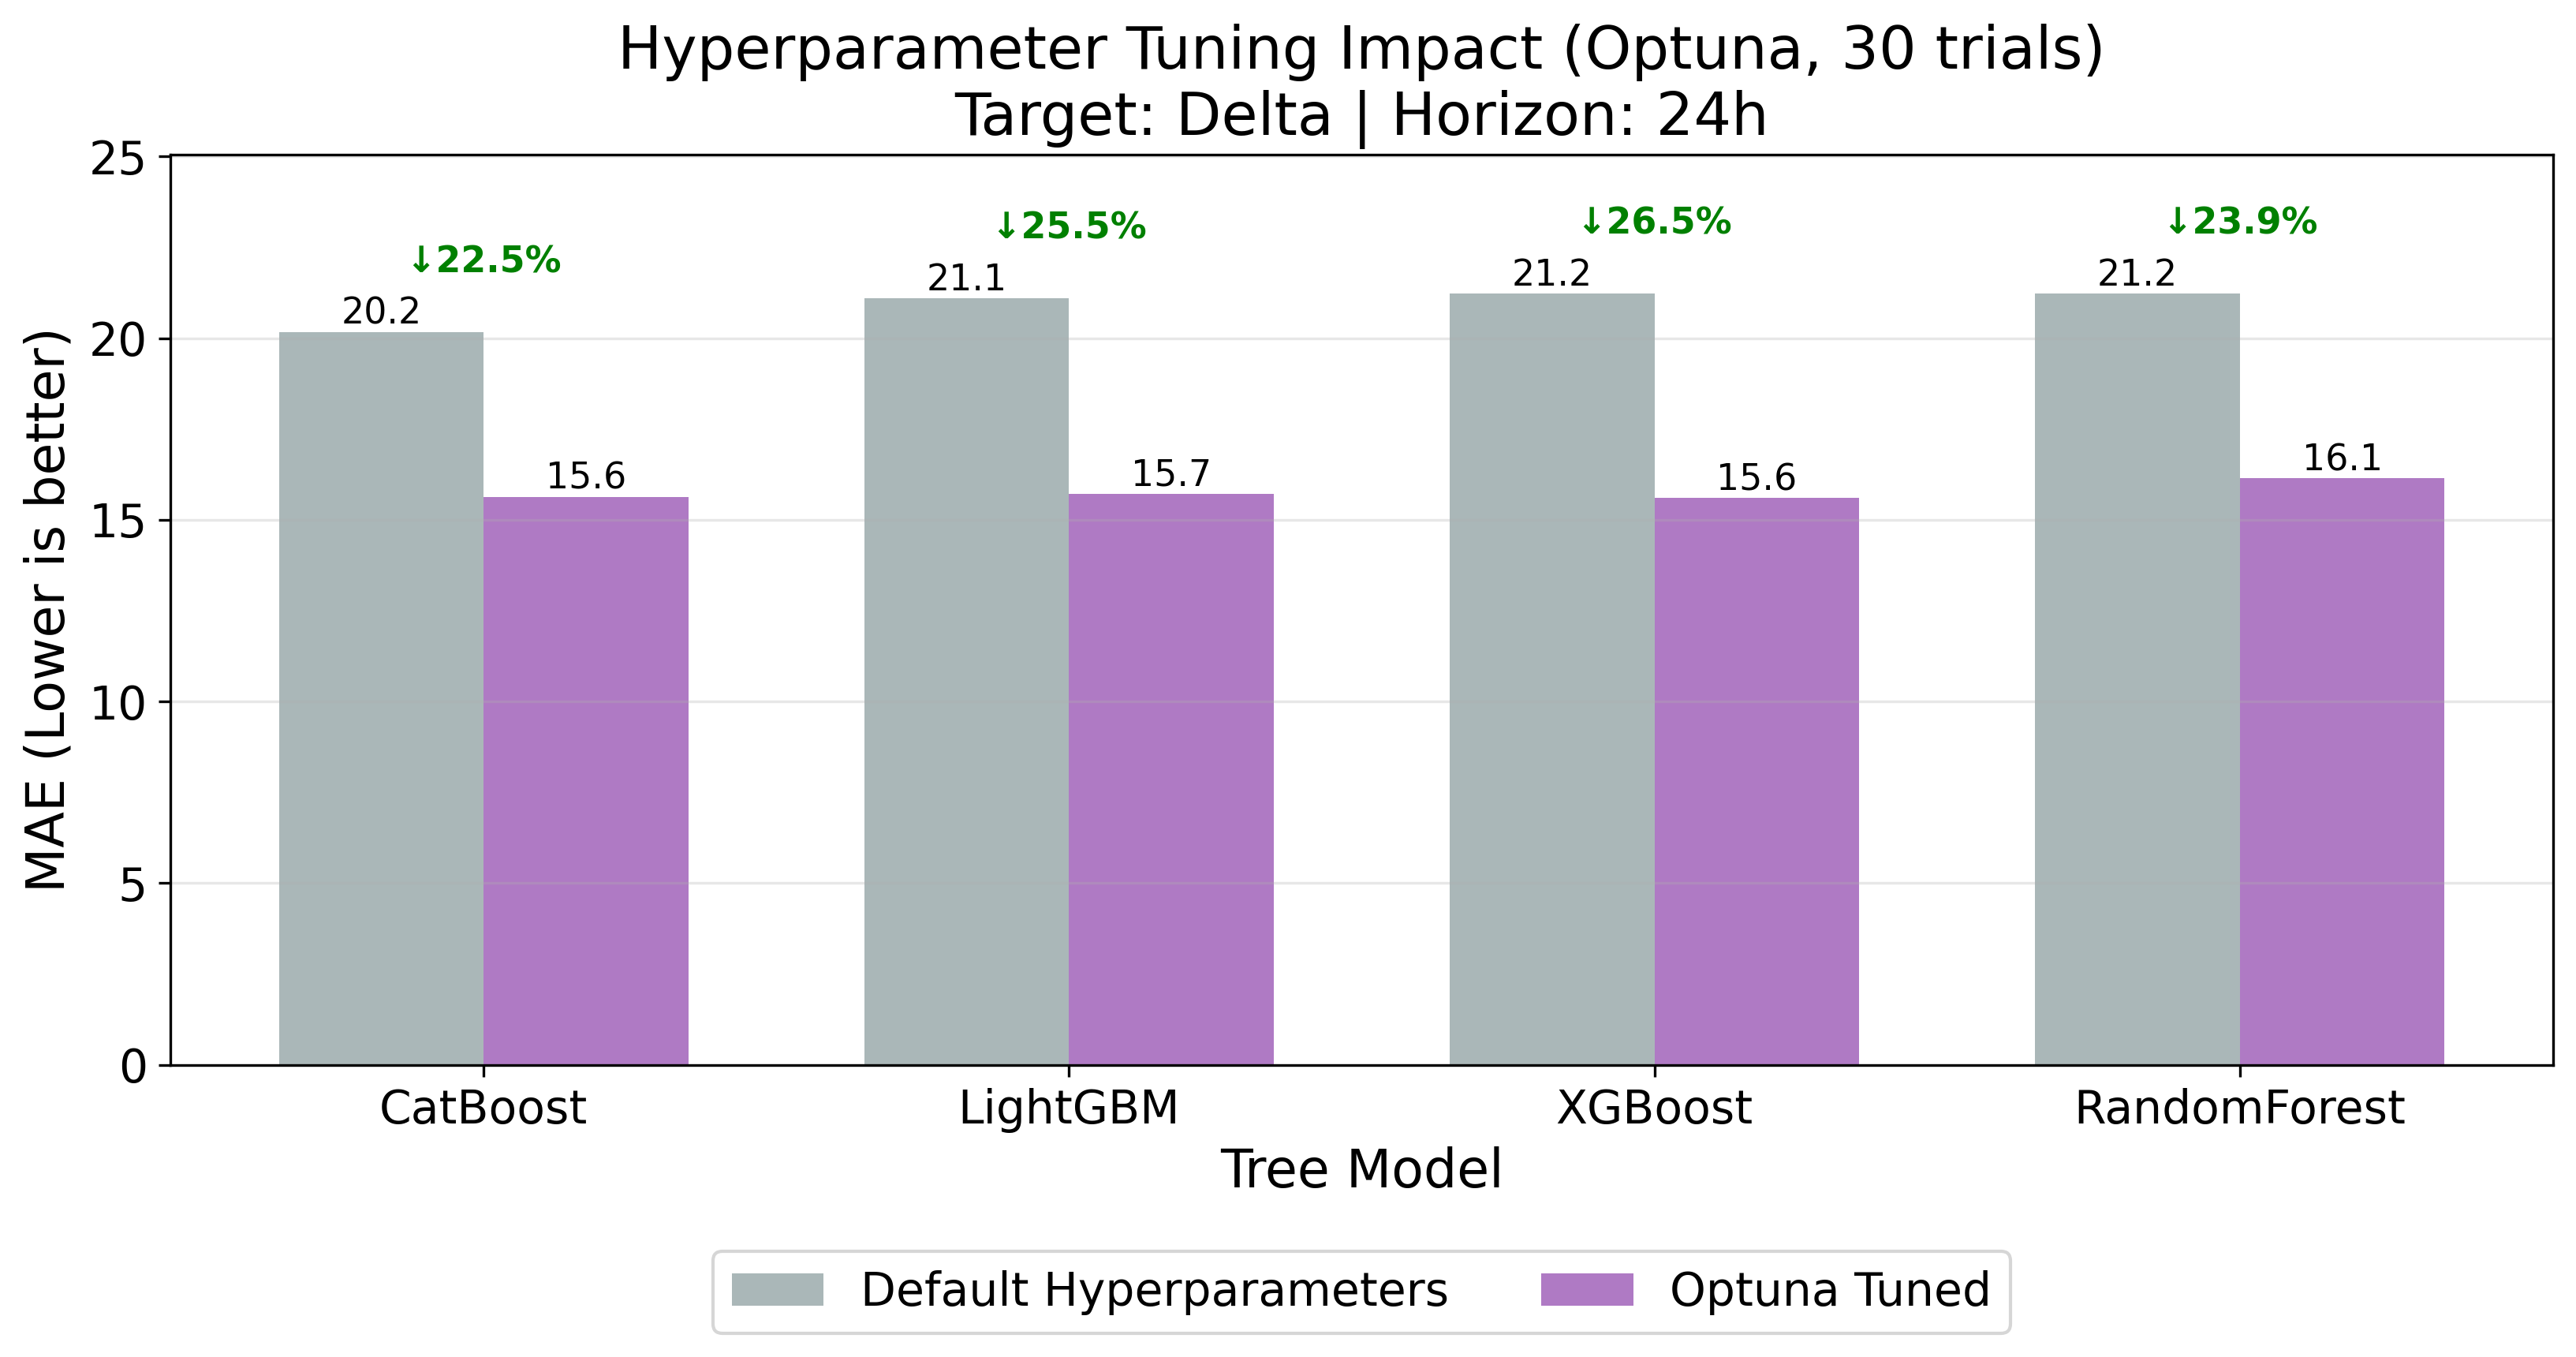
\includegraphics[width=\textwidth]{fig/Optuna_Tuning_Gain_Delta.png}
	\caption{ MAE comparisons of tree-based models when tuned by Optuna for 30 
	iterations at the 24h horizon. Lower is better.}
	\label{fig:optunaDelta}
\end{figure*}

\begin{figure*}[ht]
	\centering
	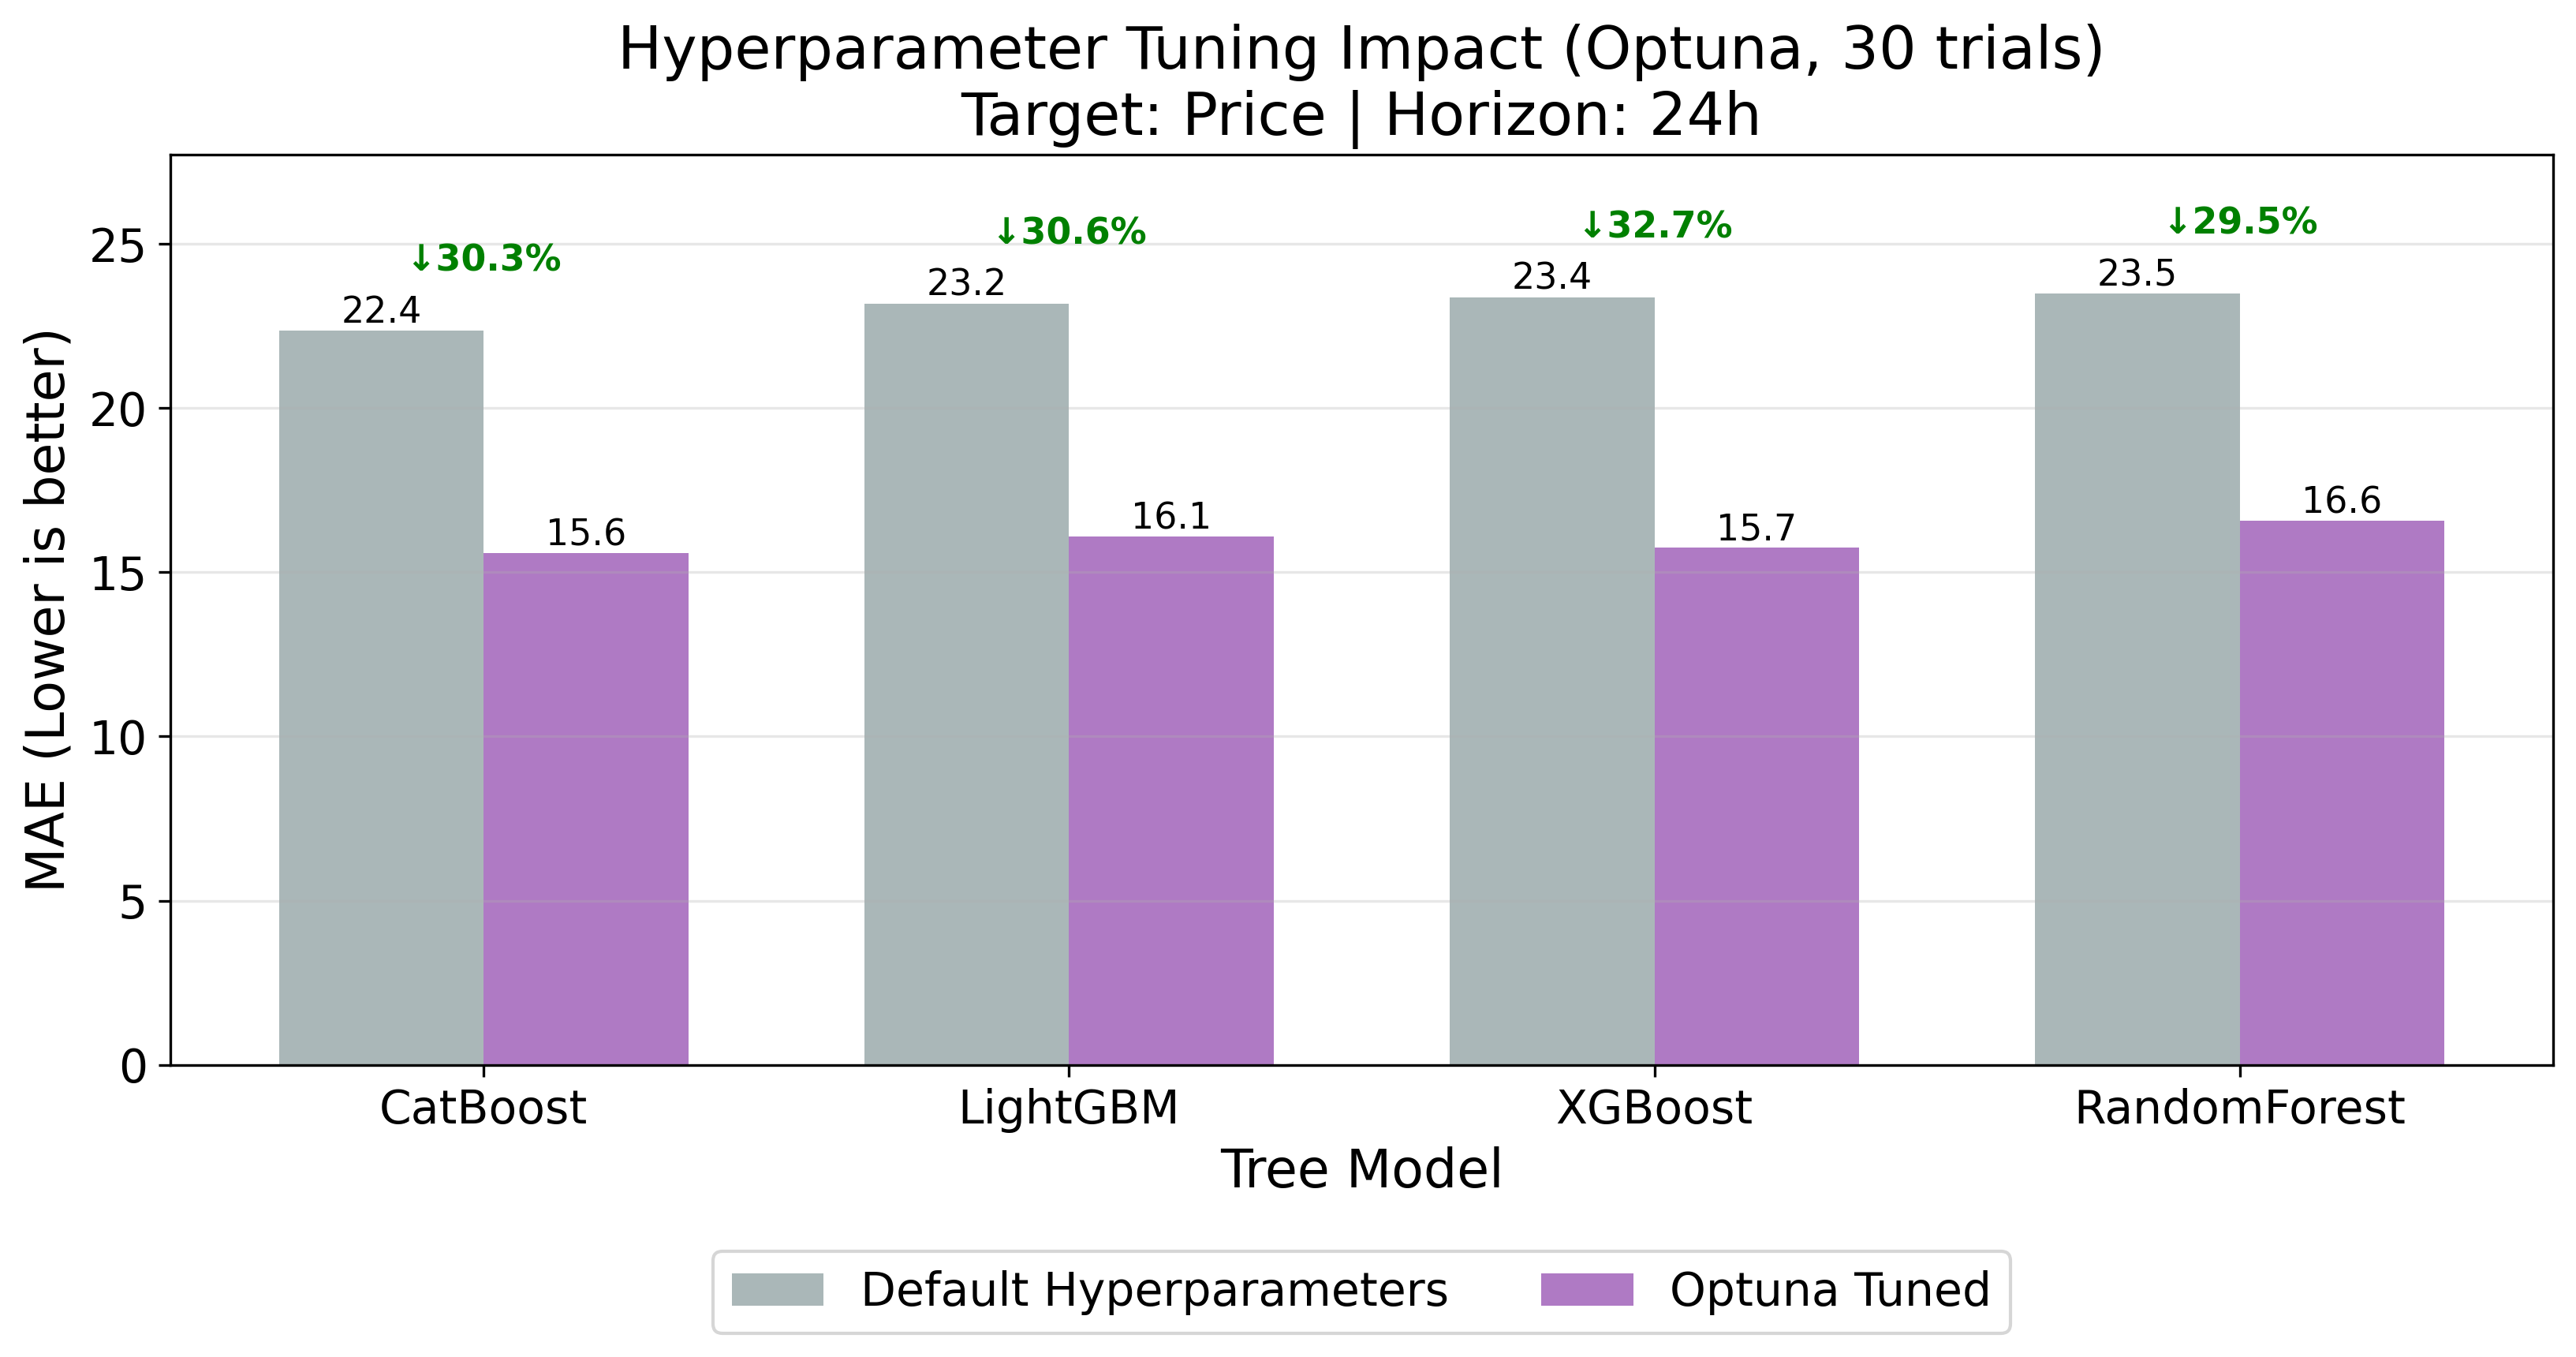
\includegraphics[width=\textwidth]{fig/Optuna_Tuning_Gain_Price.png}
	\caption{ MAE comparisons of tree-based models when tuned by Optuna for 30 
	iterations at the 24h horizon. Lower is better.}
	\label{fig:optunaPrice}
\end{figure*}

\begin{figure*}[ht]
	\centering
	
\includegraphics[width=\textwidth]{fig/Weather_Source_DMI_vs_Midas_Delta.png}
	\caption{MAE comparisons of models with and without Midas-provided weather 
	data at the 24h horizon. Lower is better.}
	\label{fig:midasAddDelta}
\end{figure*}

\begin{figure*}[ht]
	\centering
	
\includegraphics[width=\textwidth]{fig/Weather_Source_DMI_vs_Midas_Price.png}
	\caption{MAE comparisons of models with and without Midas-provided weather 
	data at the 24h horizon. Lower is better.}
	\label{fig:midasAddPrice}
\end{figure*}

\begin{figure*}[ht]
	\centering
	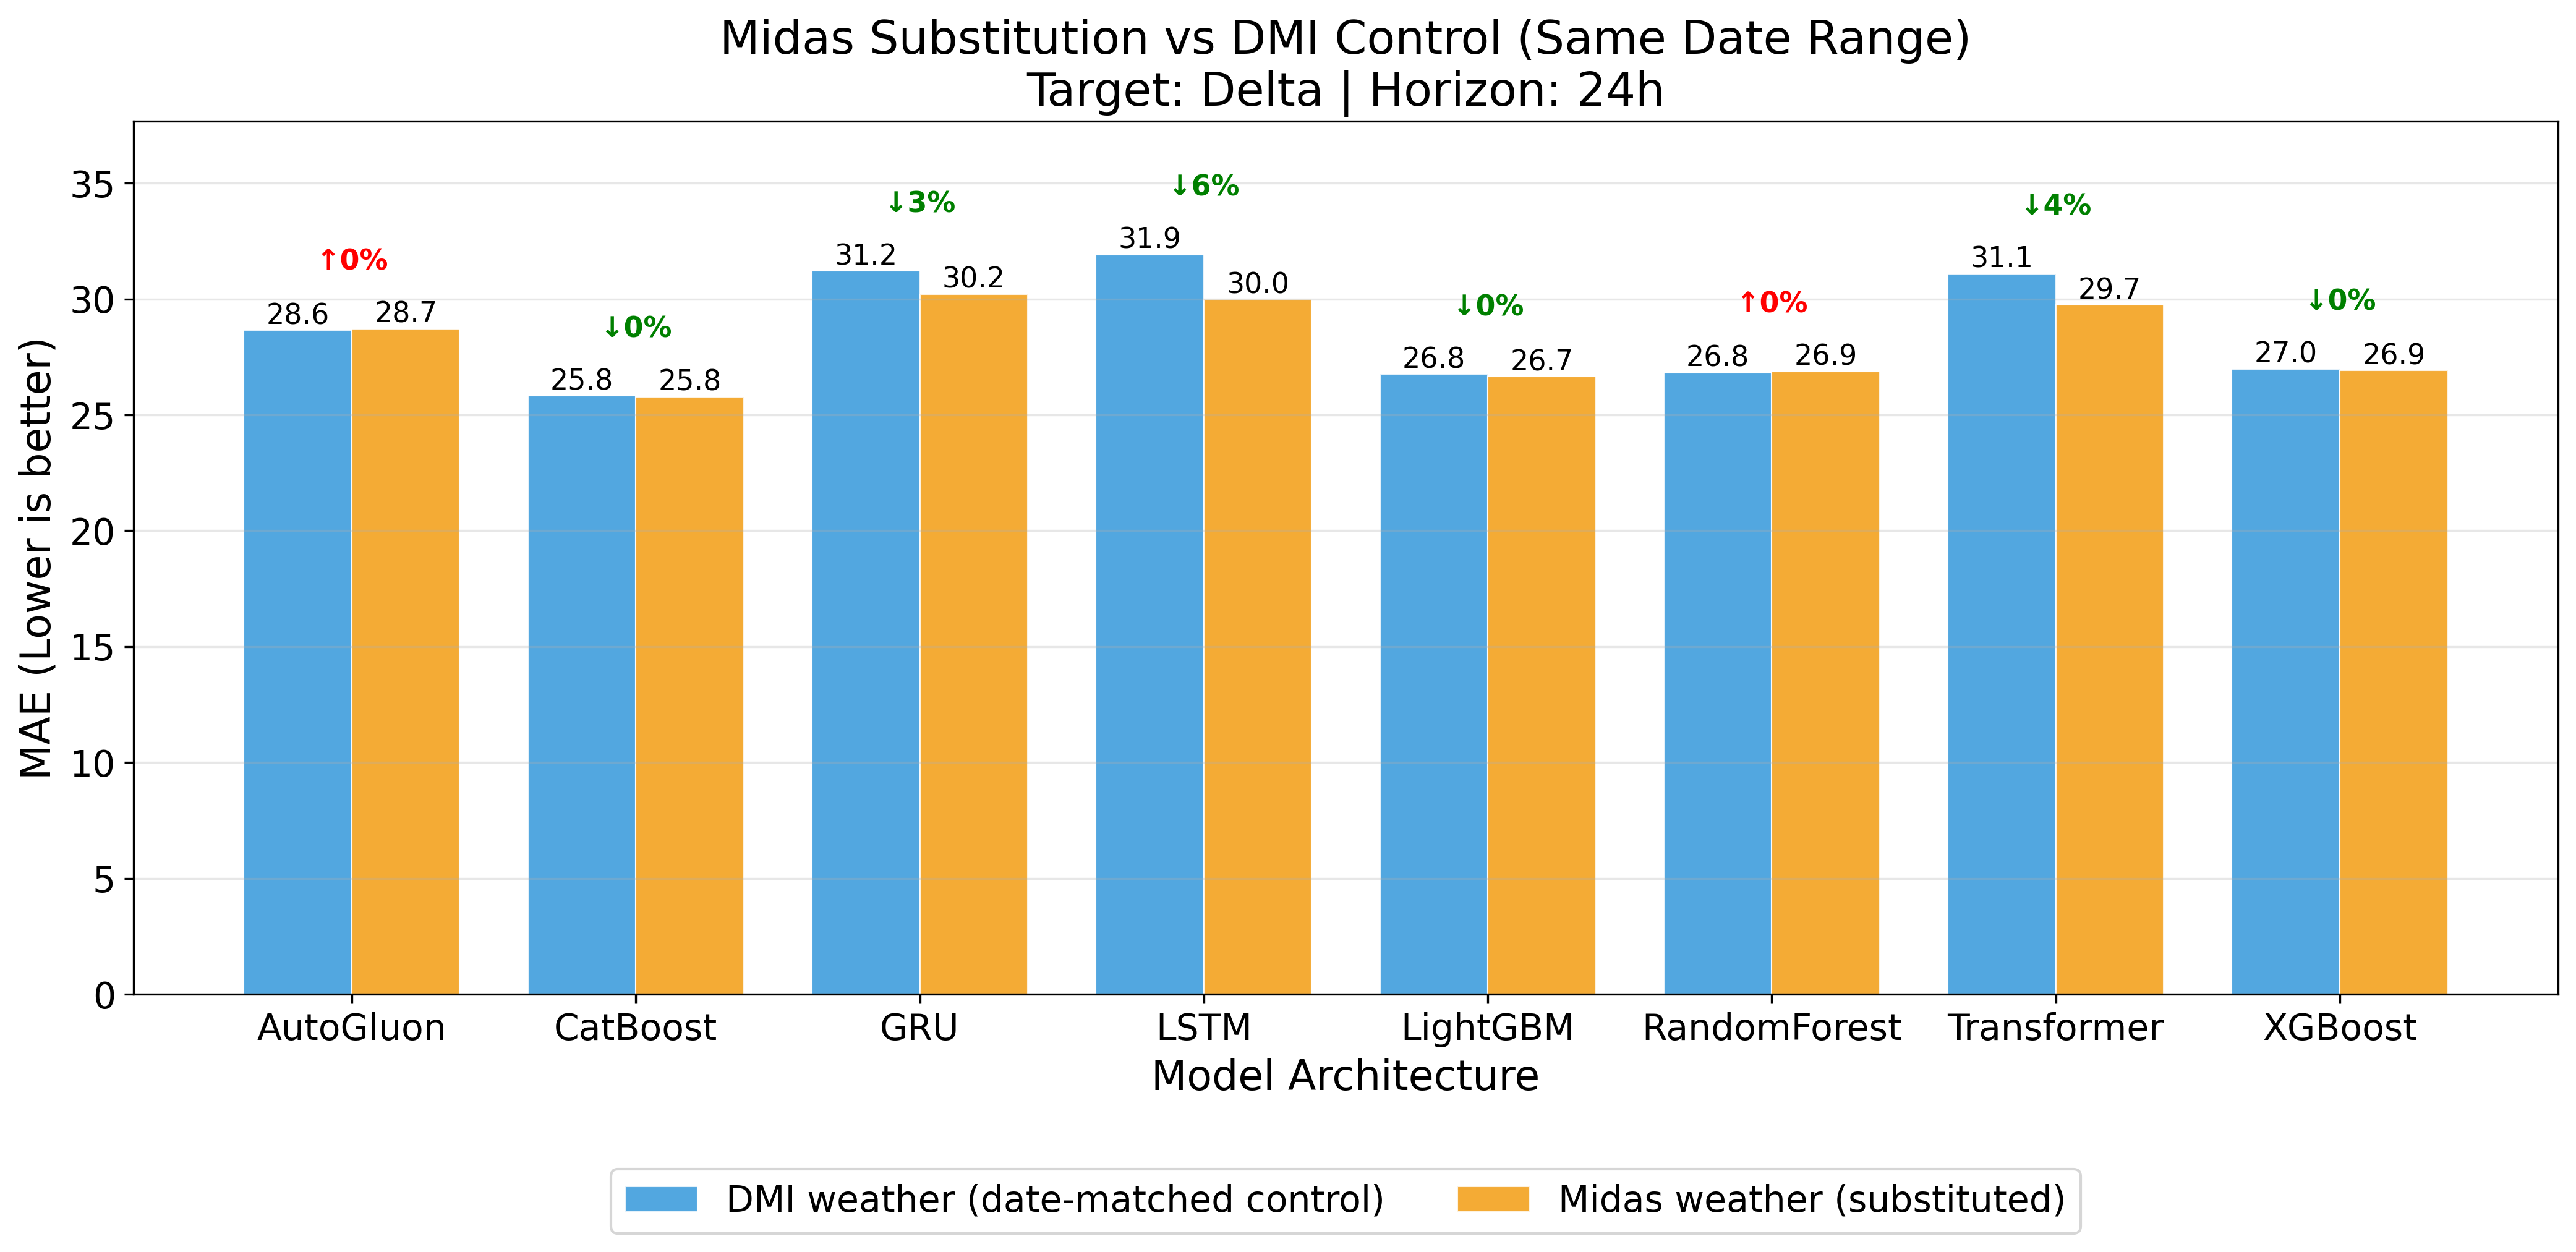
\includegraphics[width=\textwidth]{fig/Midas_Substitution_Delta.png}
	\caption{MAE comparisons of models with and without substitution of 
	original weather data with Midas-provided weather data
		at the 24h horizon. Lower is better.}
	\label{fig:midasSubDelta}
\end{figure*}

\begin{figure*}[ht]
	\centering
	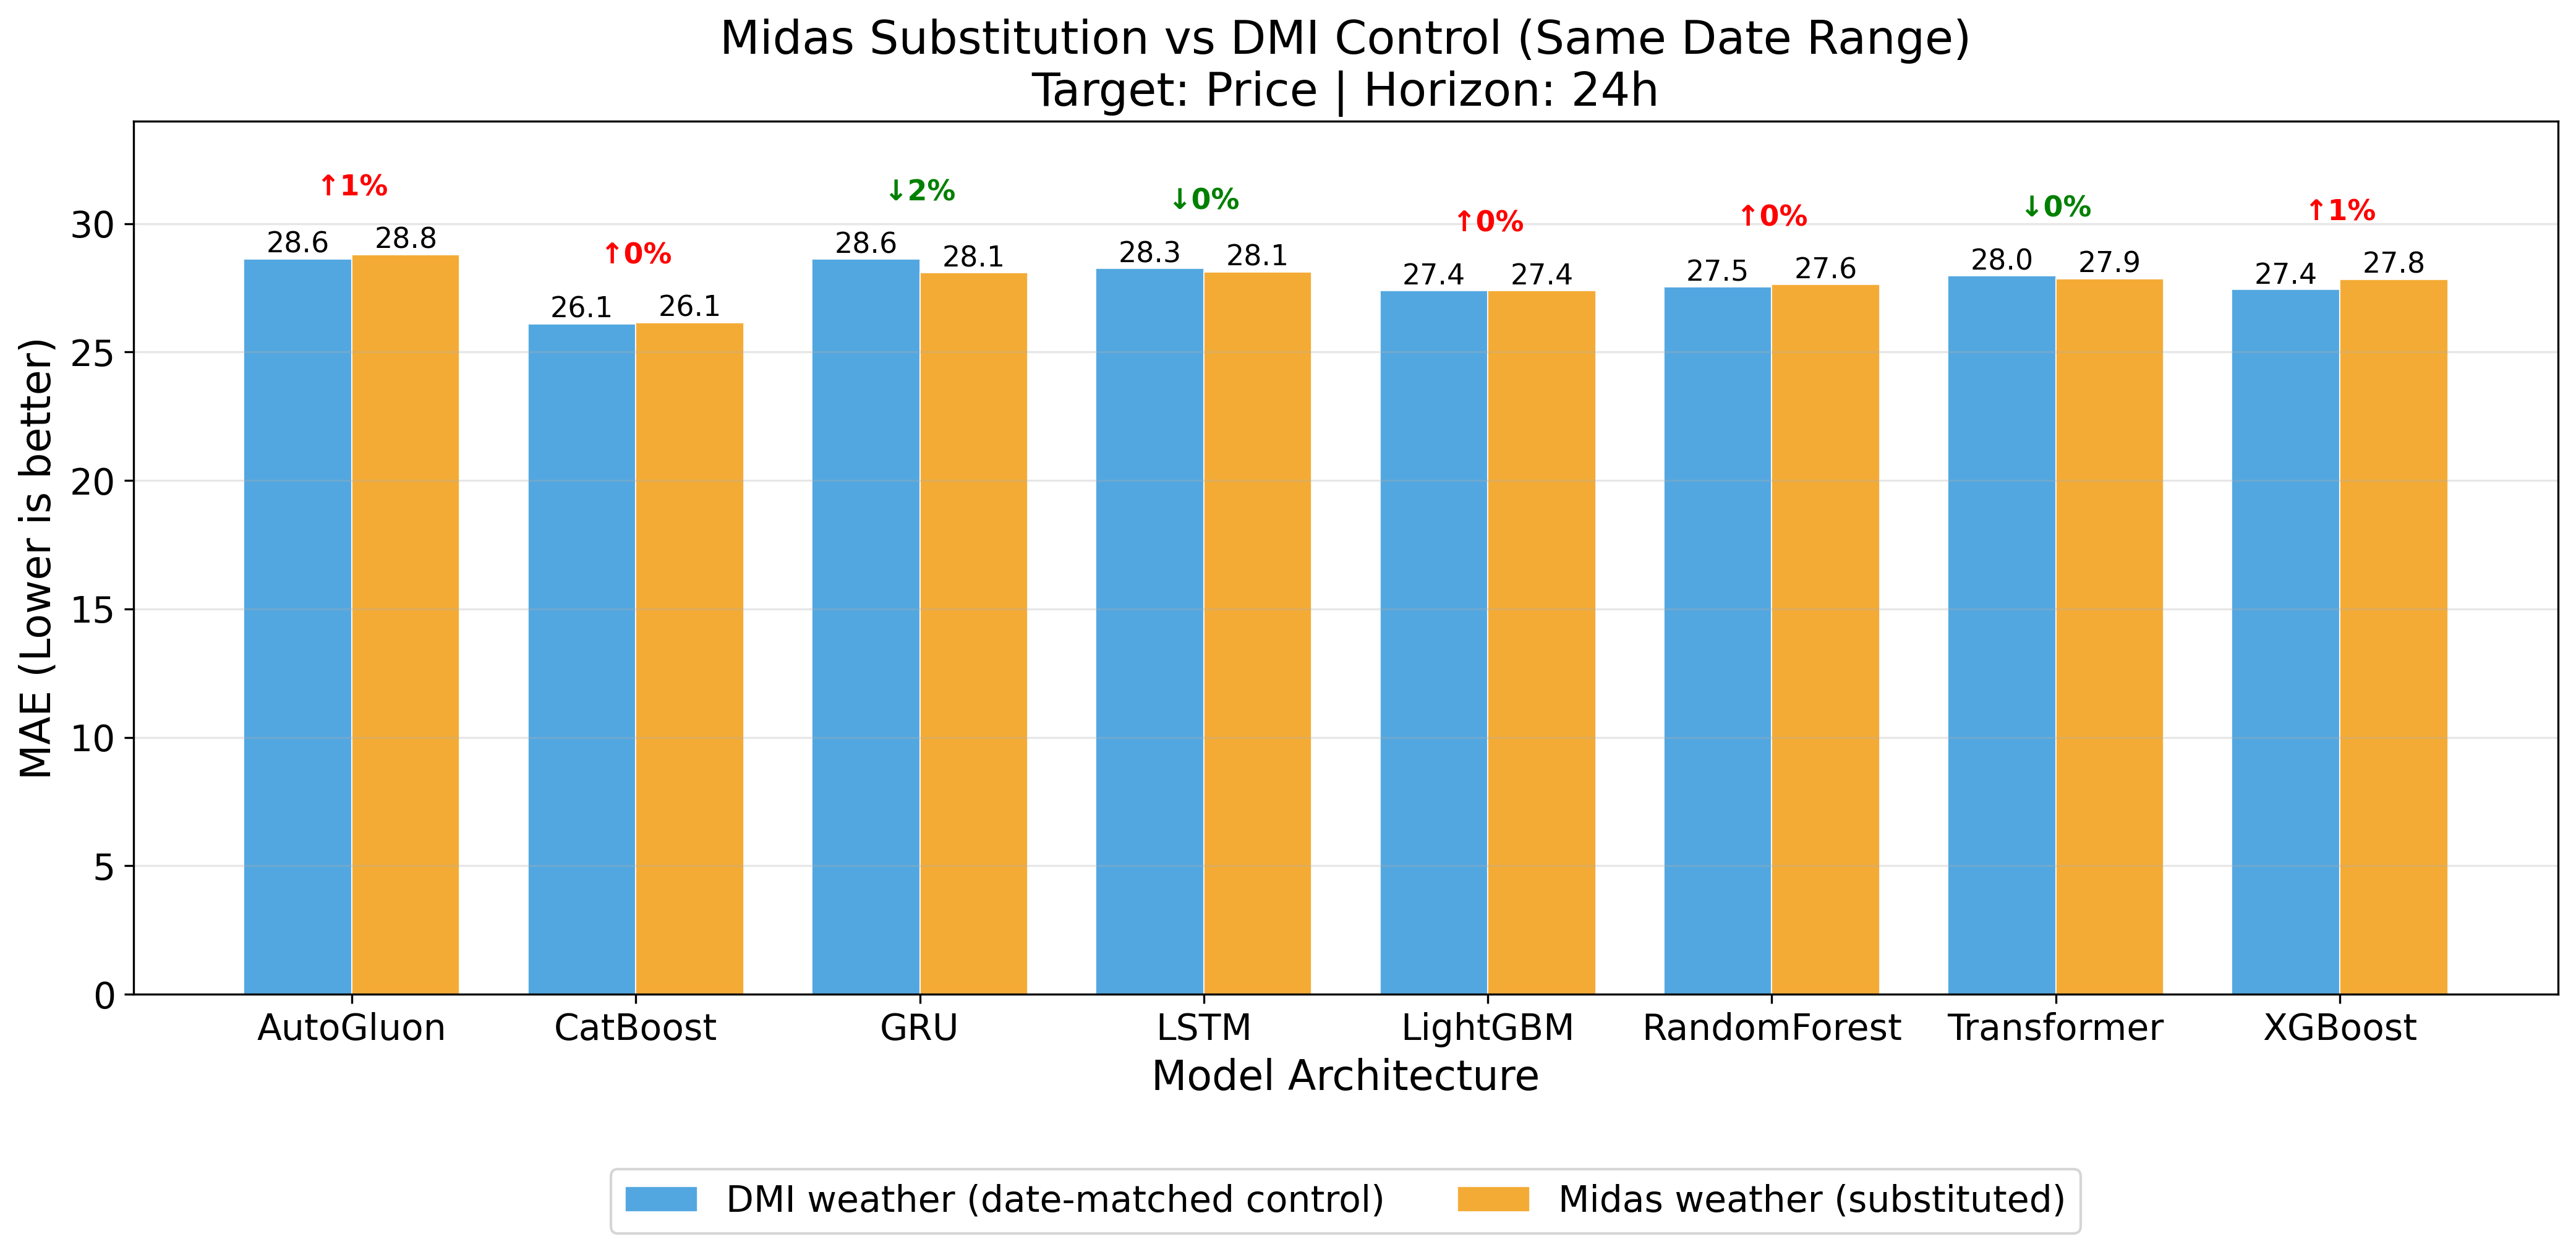
\includegraphics[width=\textwidth]{fig/Midas_Substitution_Price.png}
	\caption{MAE comparisons of models with and without substitution of 
	original weather data with Midas-provided weather data
		at the 24h horizon. Lower is better.}
	\label{fig:midasSubPrice}
\end{figure*}

\begin{figure*}[ht]
	\centering
	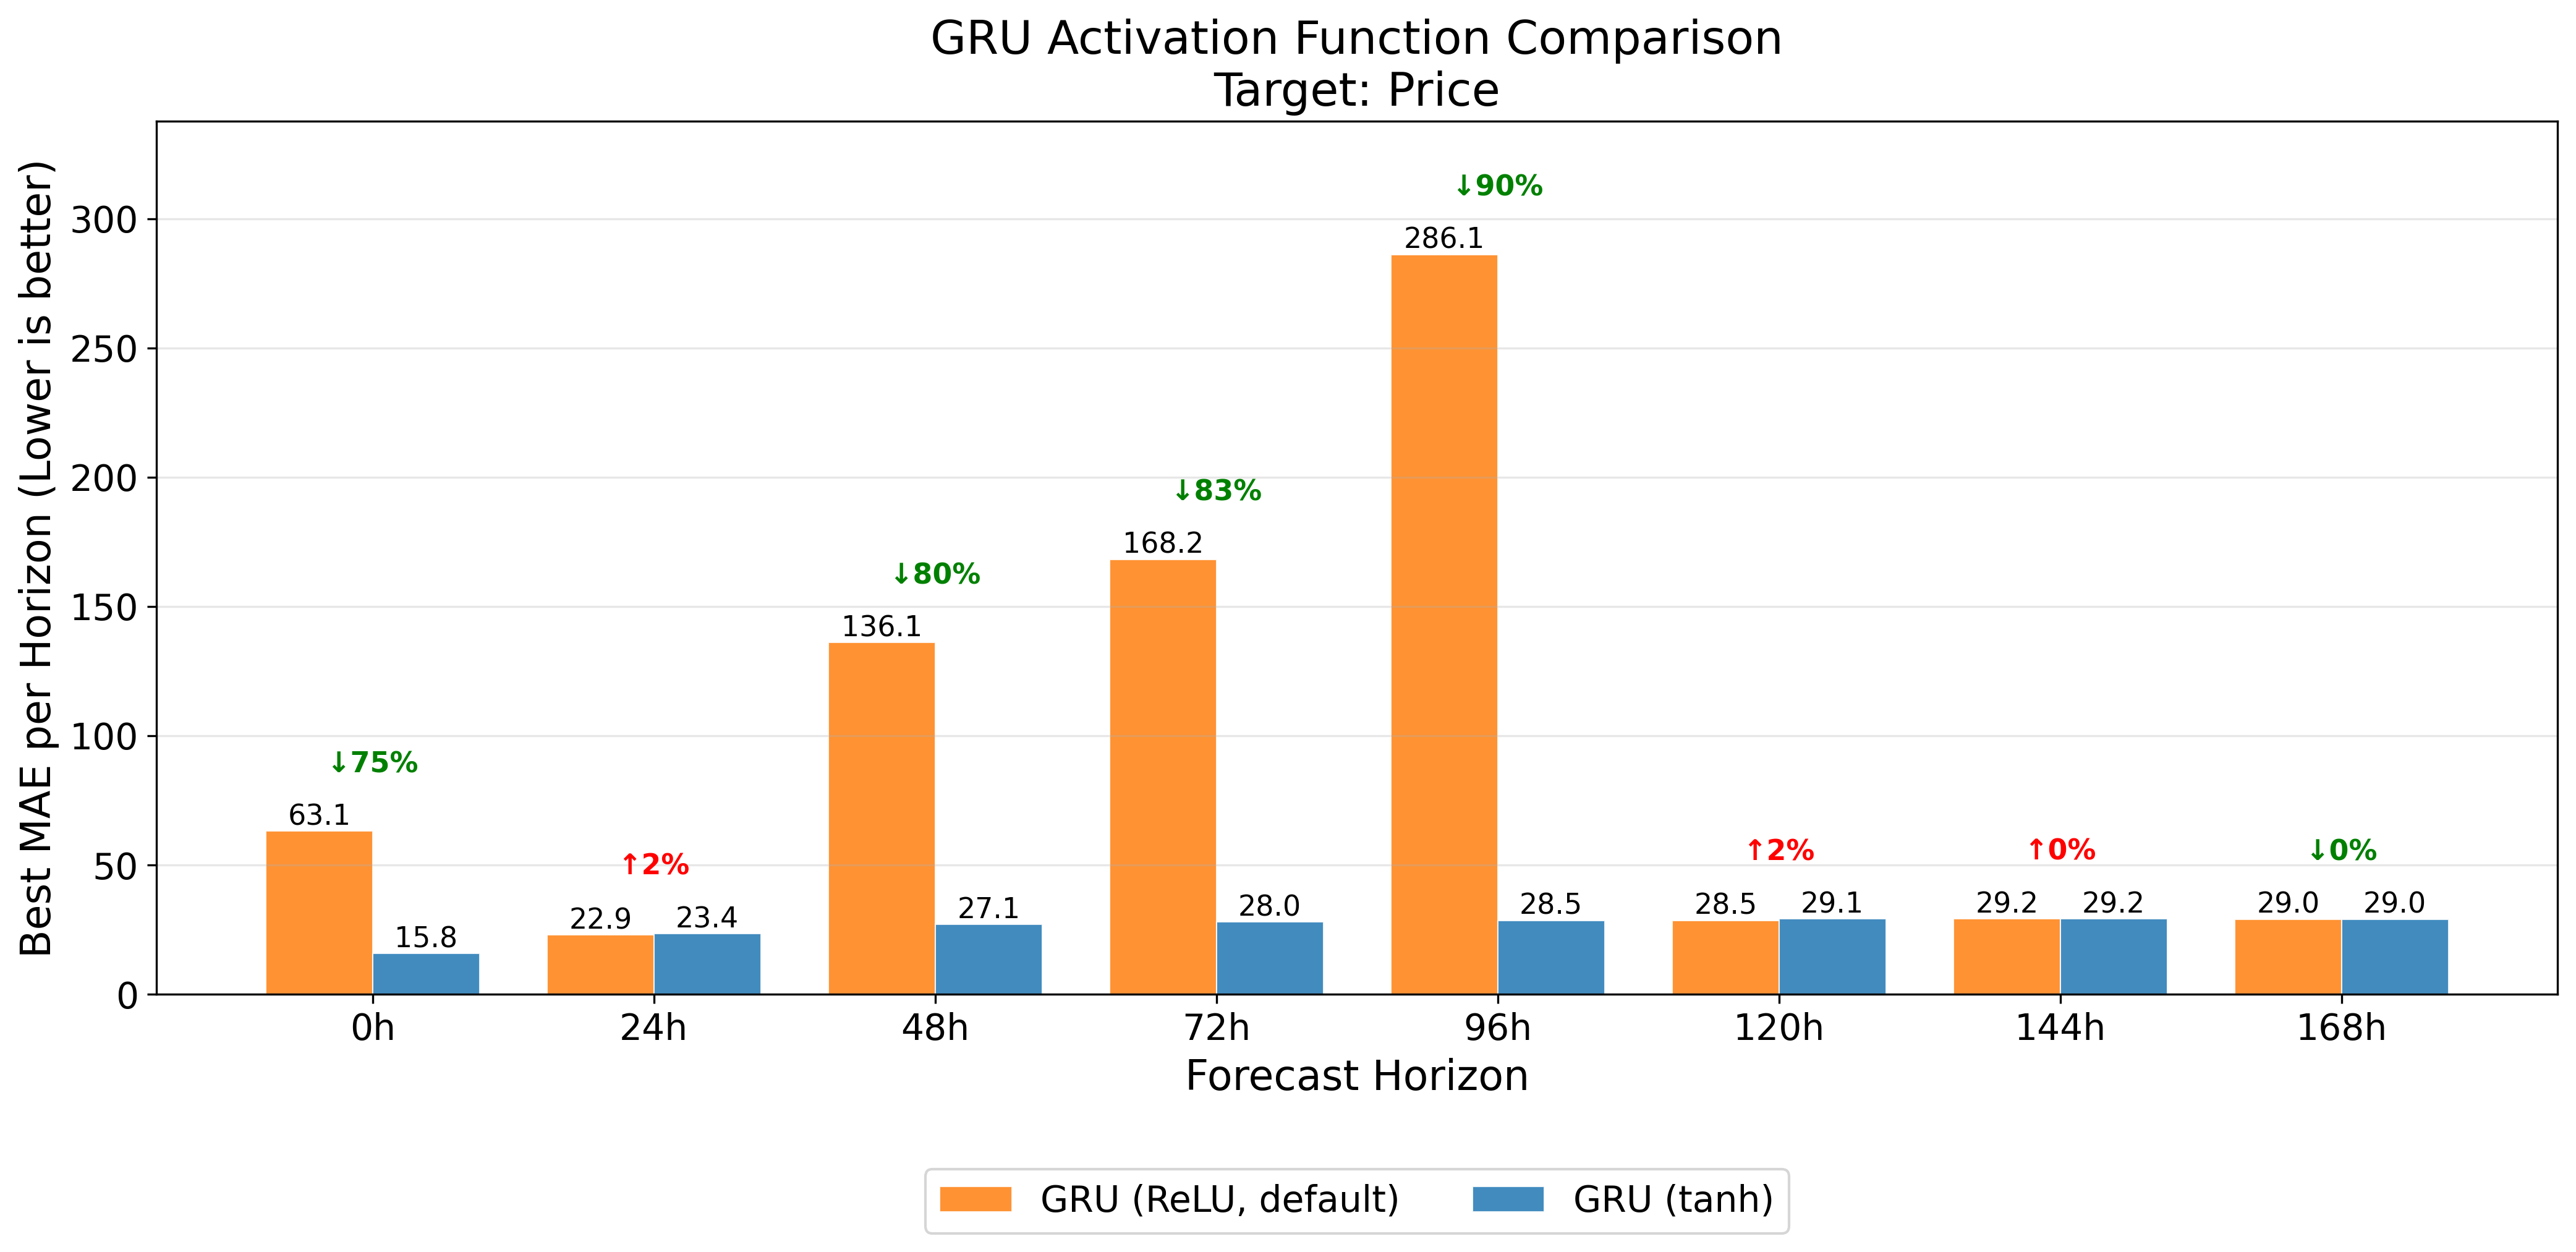
\includegraphics[width=\textwidth]{fig/GRU_Activation_Comparison_Price.png}
	\caption{MAE comparisons of GRU models with ReLU and TANH activation 
	functions. Lower is better.}
	\label{fig:gruTANH}
\end{figure*}

